\label{sec:bestresults}
The table below illustrates the lowest classification errors we were able to achieve with our decision tree, extra-tree, and LDA classifiers on the MNIST and Yale Extended B datasets. In LDA, we split the datasets in half so we can the other half for test. Using decision trees on MNIST, we utilized half of the dataset for training and half for testing. However, since the Yale B dataset is so small, we were only able to get lower error rates by using $\sim$95\% of the set for training and $\sim$5\% for testing (on decision trees.) For our best extra-tree result on MNIST, we split the dataset in half and trained 100 trees. The Yale B result comes from one of our 5-fold cross validations with 50 trees.

\begin{table}[H]
  \centering
  \begin{tabular}{||c | c | c||} 
    \hline
    Algorithm & MNIST & Yale B \\
    \hline\hline
    LDA & 13.5\%  & 6.8\% \\ 
    \hline
    Decision Tree & 16.6\% & 57.89\% \\ 
    \hline
    Extra-Trees & 4.89\% & 34.02\% \\
    \hline
  \end{tabular}
  \caption{Lowest classification errors achieved with LDA, Decision Trees, and Extra-Trees.}
\end{table}

\subsection{Cross Validation}

In an effort to justify our choice of hyperparameters and examine the stability of our classifiers irrespective of variations in the training and test sets, we performed a 5-fold cross validation across the tuning parameters in each algorithm. For decision and extra trees, this consists of \code{minLeaf}. Future implementations could include more complex parameters. In $k$-fold cross validation, $k$ classifiers are trained on different subsets of the entire set, ensuring that each sample of the dataset is used only once for validation. This helps to mitigate the effects of variation in the dataset and illustrate the general performance of the classifier at hand. The $k$ classifiers' error rates are averaged to give a strong estimate of the algorithm's true performance. The figure below illustrates this process for $k=4$.  
%
\begin{figure}[H]
  \centering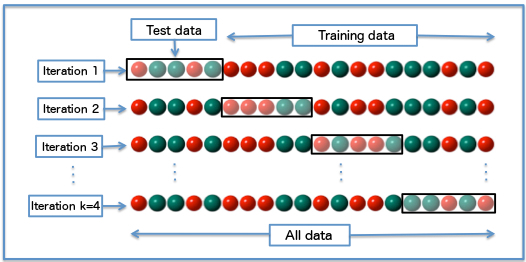
\includegraphics[width=0.6\columnwidth]{../images/K-fold_cross_validation_EN}
  \caption{4-fold cross validation on a dataset.}
\end{figure}
 
The best results of our cross validation are represented in the table below. The error rates are averaged over the 5 folds. Note that because the 5-fold cross validation yields a larger test set for Yale B than in previous results (\cref{sec:bestresults}), the error rate for decision trees on the Yale B dataset was higher. If we used a higher-fold cross validation, the results would have been better.
%
\begin{table}[H]
  \centering
  \begin{tabular}{||c | c | c||} 
    \hline
    Algorithm & MNIST & Yale B \\
    \hline\hline
    LDA & \%  & \% \\ 
    \hline
    Decision Tree & 17.9\% (\code{minLeaf = 1}) & 74.9\% (\code{minLeaf = 1})\\ 
    \hline
    Extra-Trees & 5.4\% (100 extra-trees) & 36.3\% (100 extra-trees) \\
    \hline
  \end{tabular}
  \caption{Average classification errors achieved with LDA, Decision Trees, and Extra-Trees after Cross Validation.}
\end{table}

\subsection{Hyperparameter Optimization}

\subsubsection{Decision Trees}

The figure below represents the accuracy and time performance of our decision tree algorithm on MNIST and Yale B after averaging with cross validation. Using cross validation allows us to generalize the effects of our changing hyperparameter, \code{minLeaf}, which is a value that defines the minimum number of samples required to make a leaf node in the tree. As soon as the set is split to a level below \code{minLeaf}, a class label is applied as the \emph{mode} of the samples in the set.

Note that the timing results for MNIST have high variability. This is because we ran our tests on a shared server that was at high occupancy. In this way, training our decision trees on MNIST was impacted by the other users. On our local computers, the decision tree was training in about 4 minutes, with a clear correlation between \code{minLeaf} and the time it took to complete. This process is evinced in the figure for the Yale B dataset, which was interrupted less on the server.

Our cross-validated results indicate that the highest accuracy is achieved by setting \code{minLeaf = 1}.
%
\begin{figure}[H]
    \centering
    \subfloat[]{{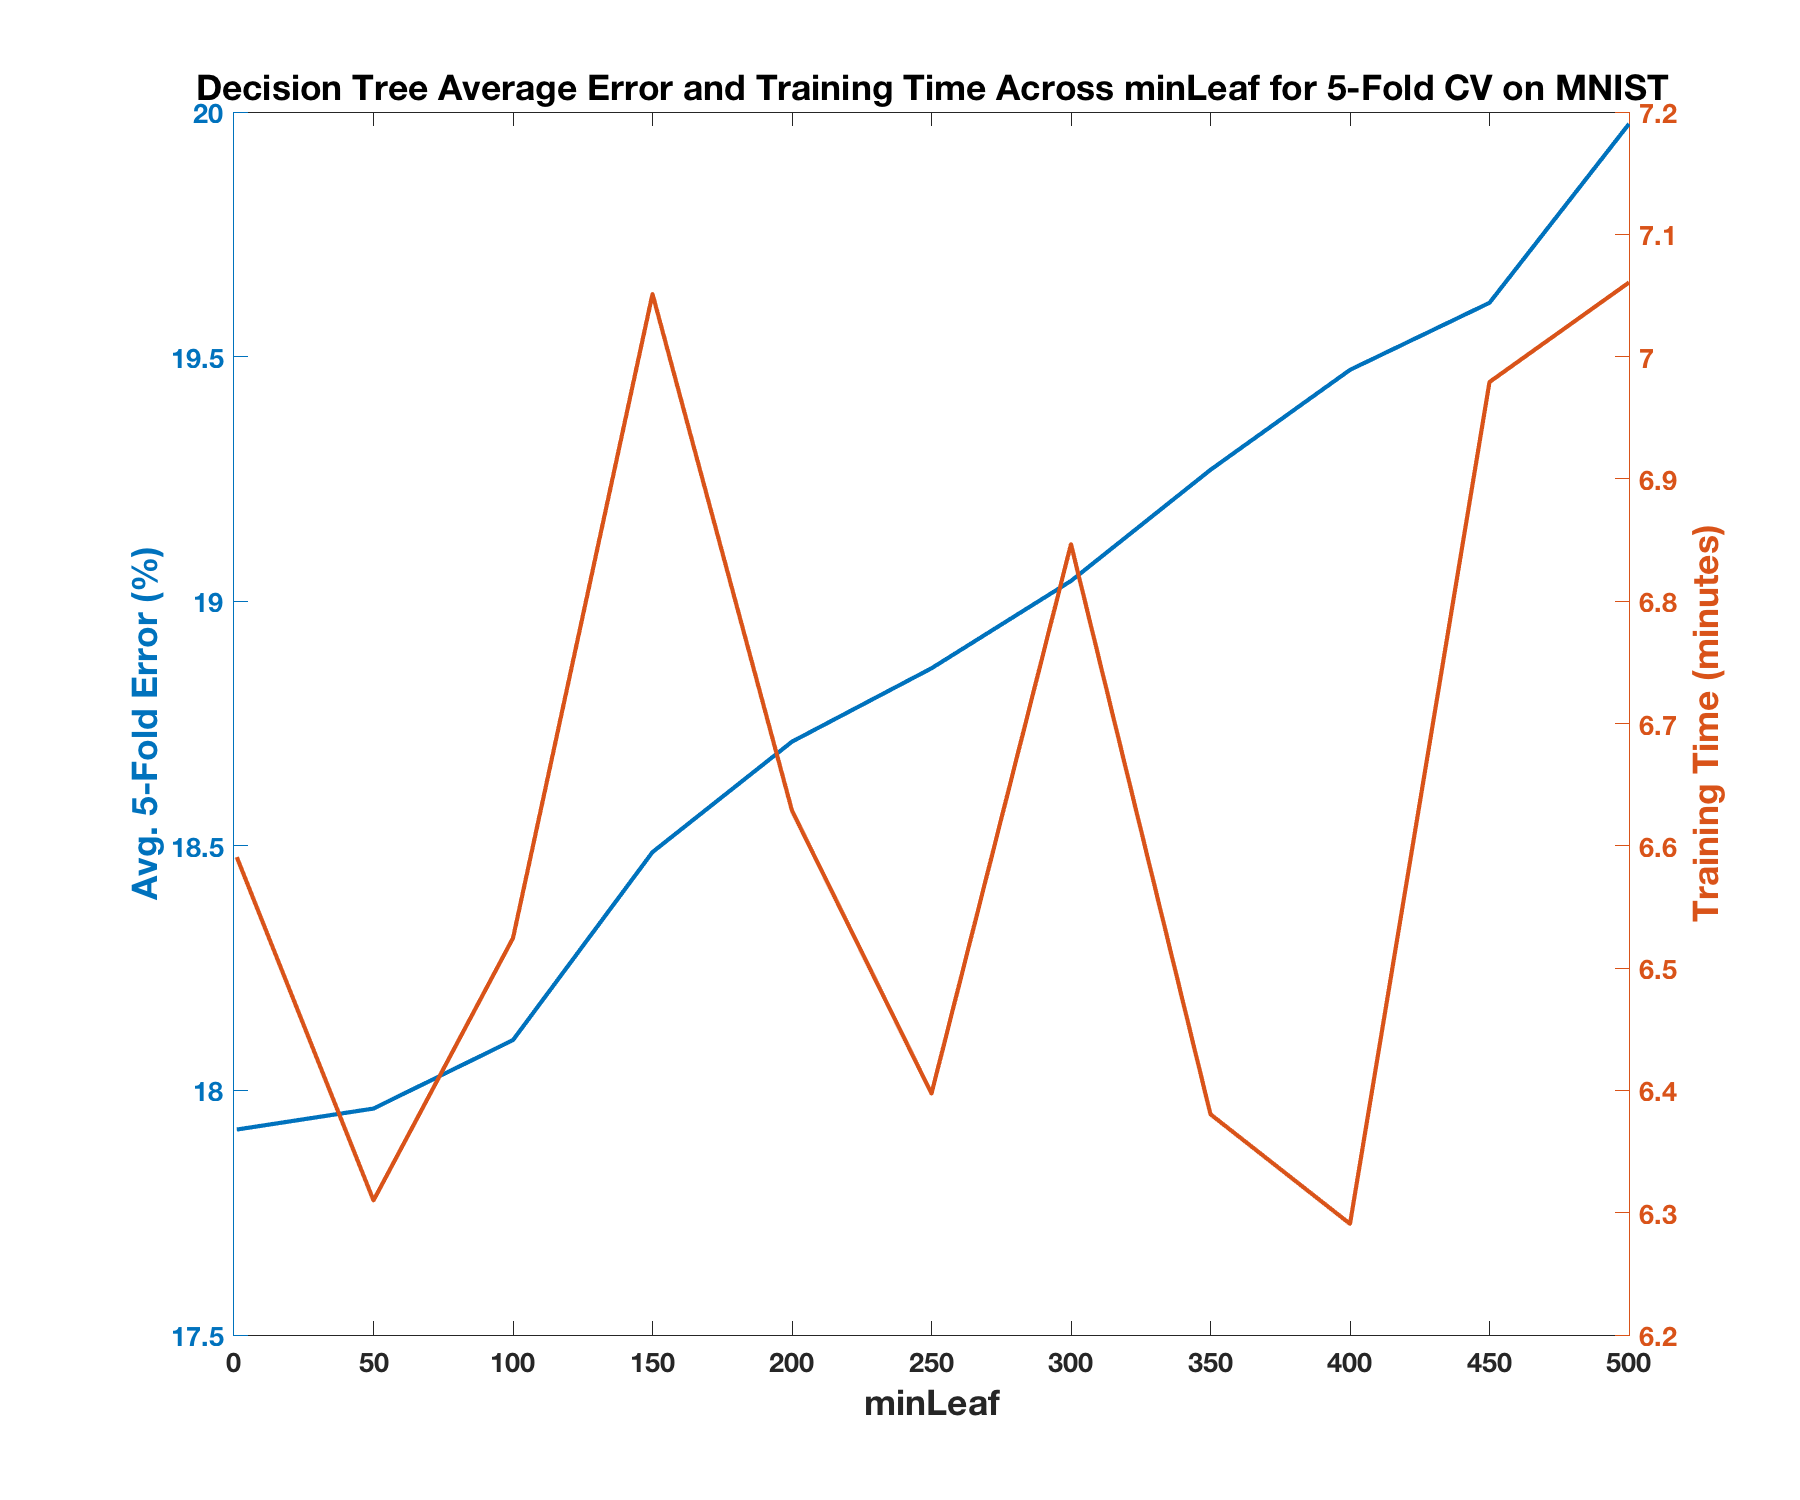
\includegraphics[width=0.5\columnwidth]{../images/cv_dt_mnist} }}
    \subfloat[]{{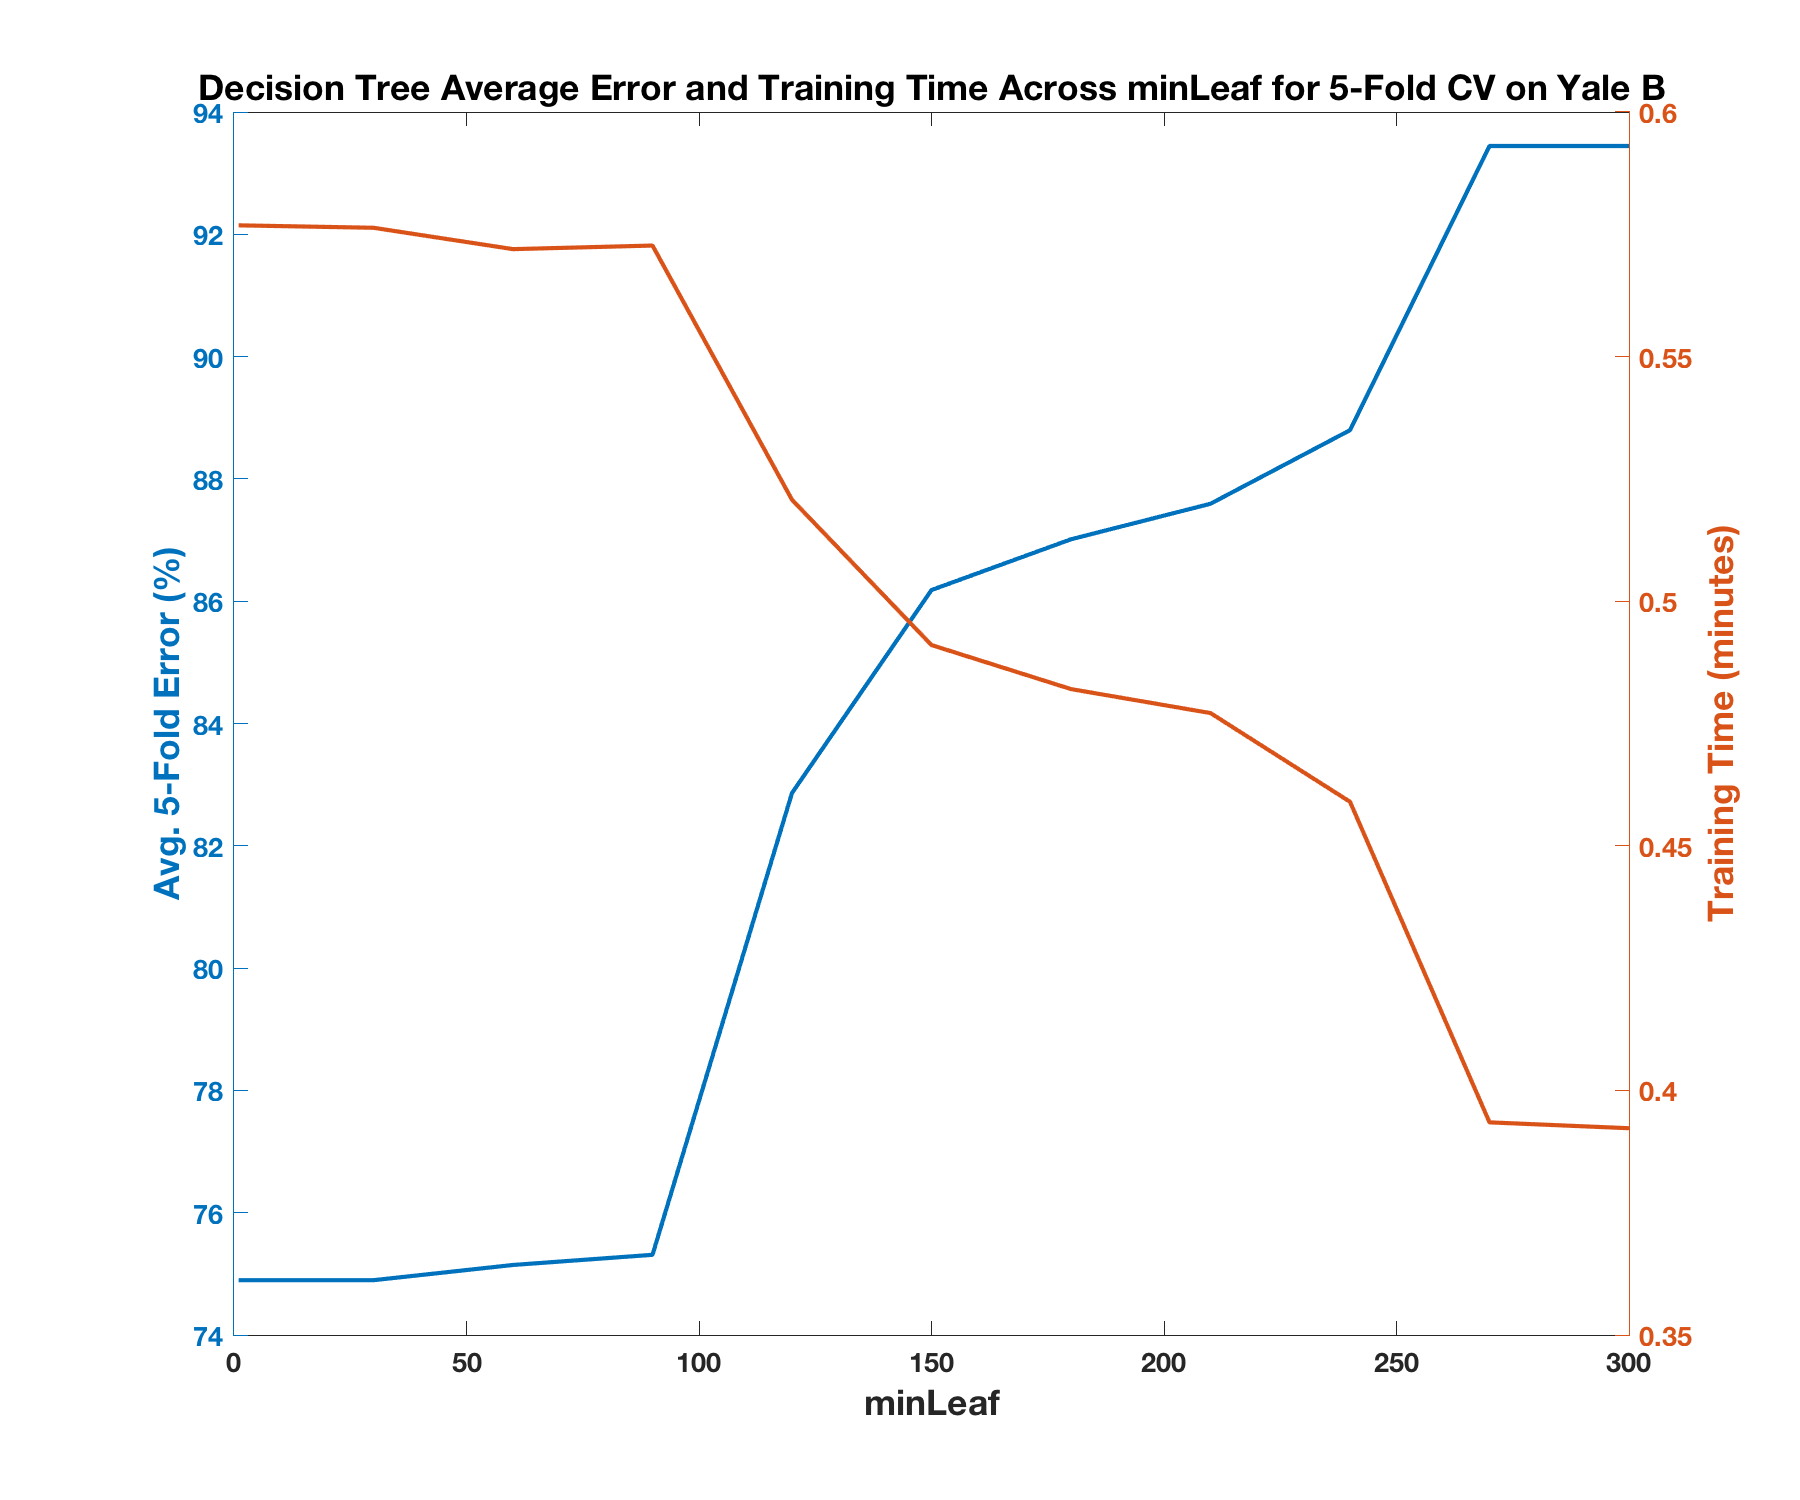
\includegraphics[width=0.5\columnwidth]{../images/cv_dt_yaleb} }}
    \caption{Cross Validated Decision Tree Hyperparameter Results on MNIST (a) and Yale B (b).}
\end{figure}

\subsubsection{Extra Trees}

The figure below represents the accuracy and time performance of our extra-tree classifier on MNIST and Yale B after averaging with cross validation. Using cross validation allows us to generalize the effects of our changing hyperparameter, \code{numTrees}, which is a value that defines the number of trees used for the ensemble. In general, more trees to vote on the classification label improves the results. Though a clear case of diminishing returns is observed after \code{numTrees = 50}.

Note that the time to train the extra-trees increases linearly with the number of trees, as the training of a decision tree, especially in the random case, is of constant time complexity. This does not include the testing of trees, which increases as $O(numTrees\ast \log n)$. This is derived by considering that \textit{numTrees} trees must be passed through to decide a class label, which takes $\log n$ time.

Our cross-validated results indicate that the highest accuracy is achieved by setting \code{numTrees > 50}, with \code{numTrees = 100} being a good compromise between time to execute and accuracy.
%
\begin{figure}[H]
    \centering
    \subfloat[]{{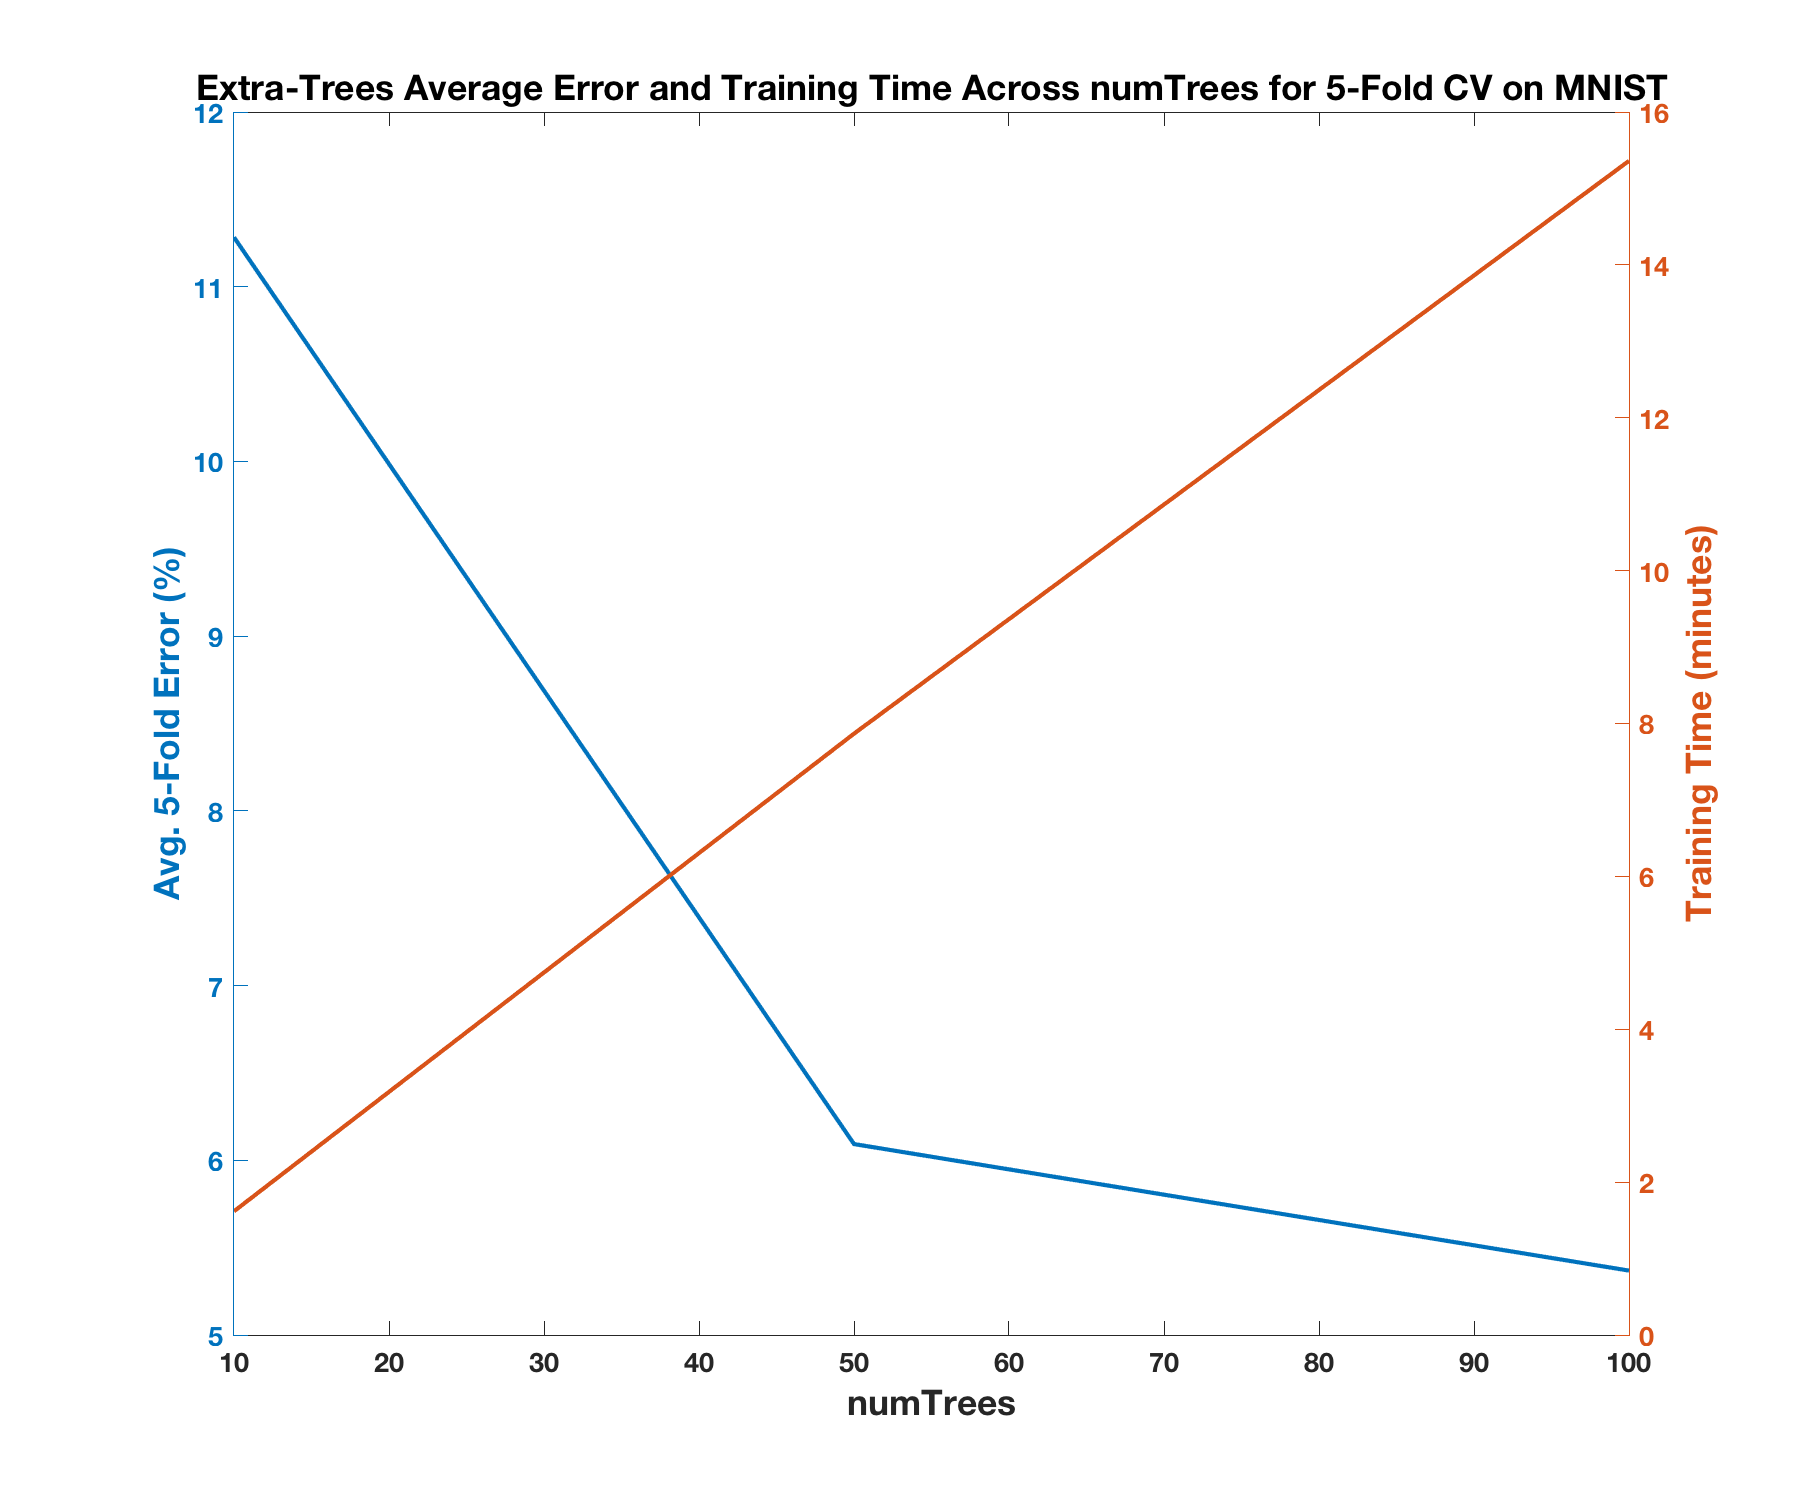
\includegraphics[width=0.5\columnwidth]{../images/cv_et_mnist} }}
    \subfloat[]{{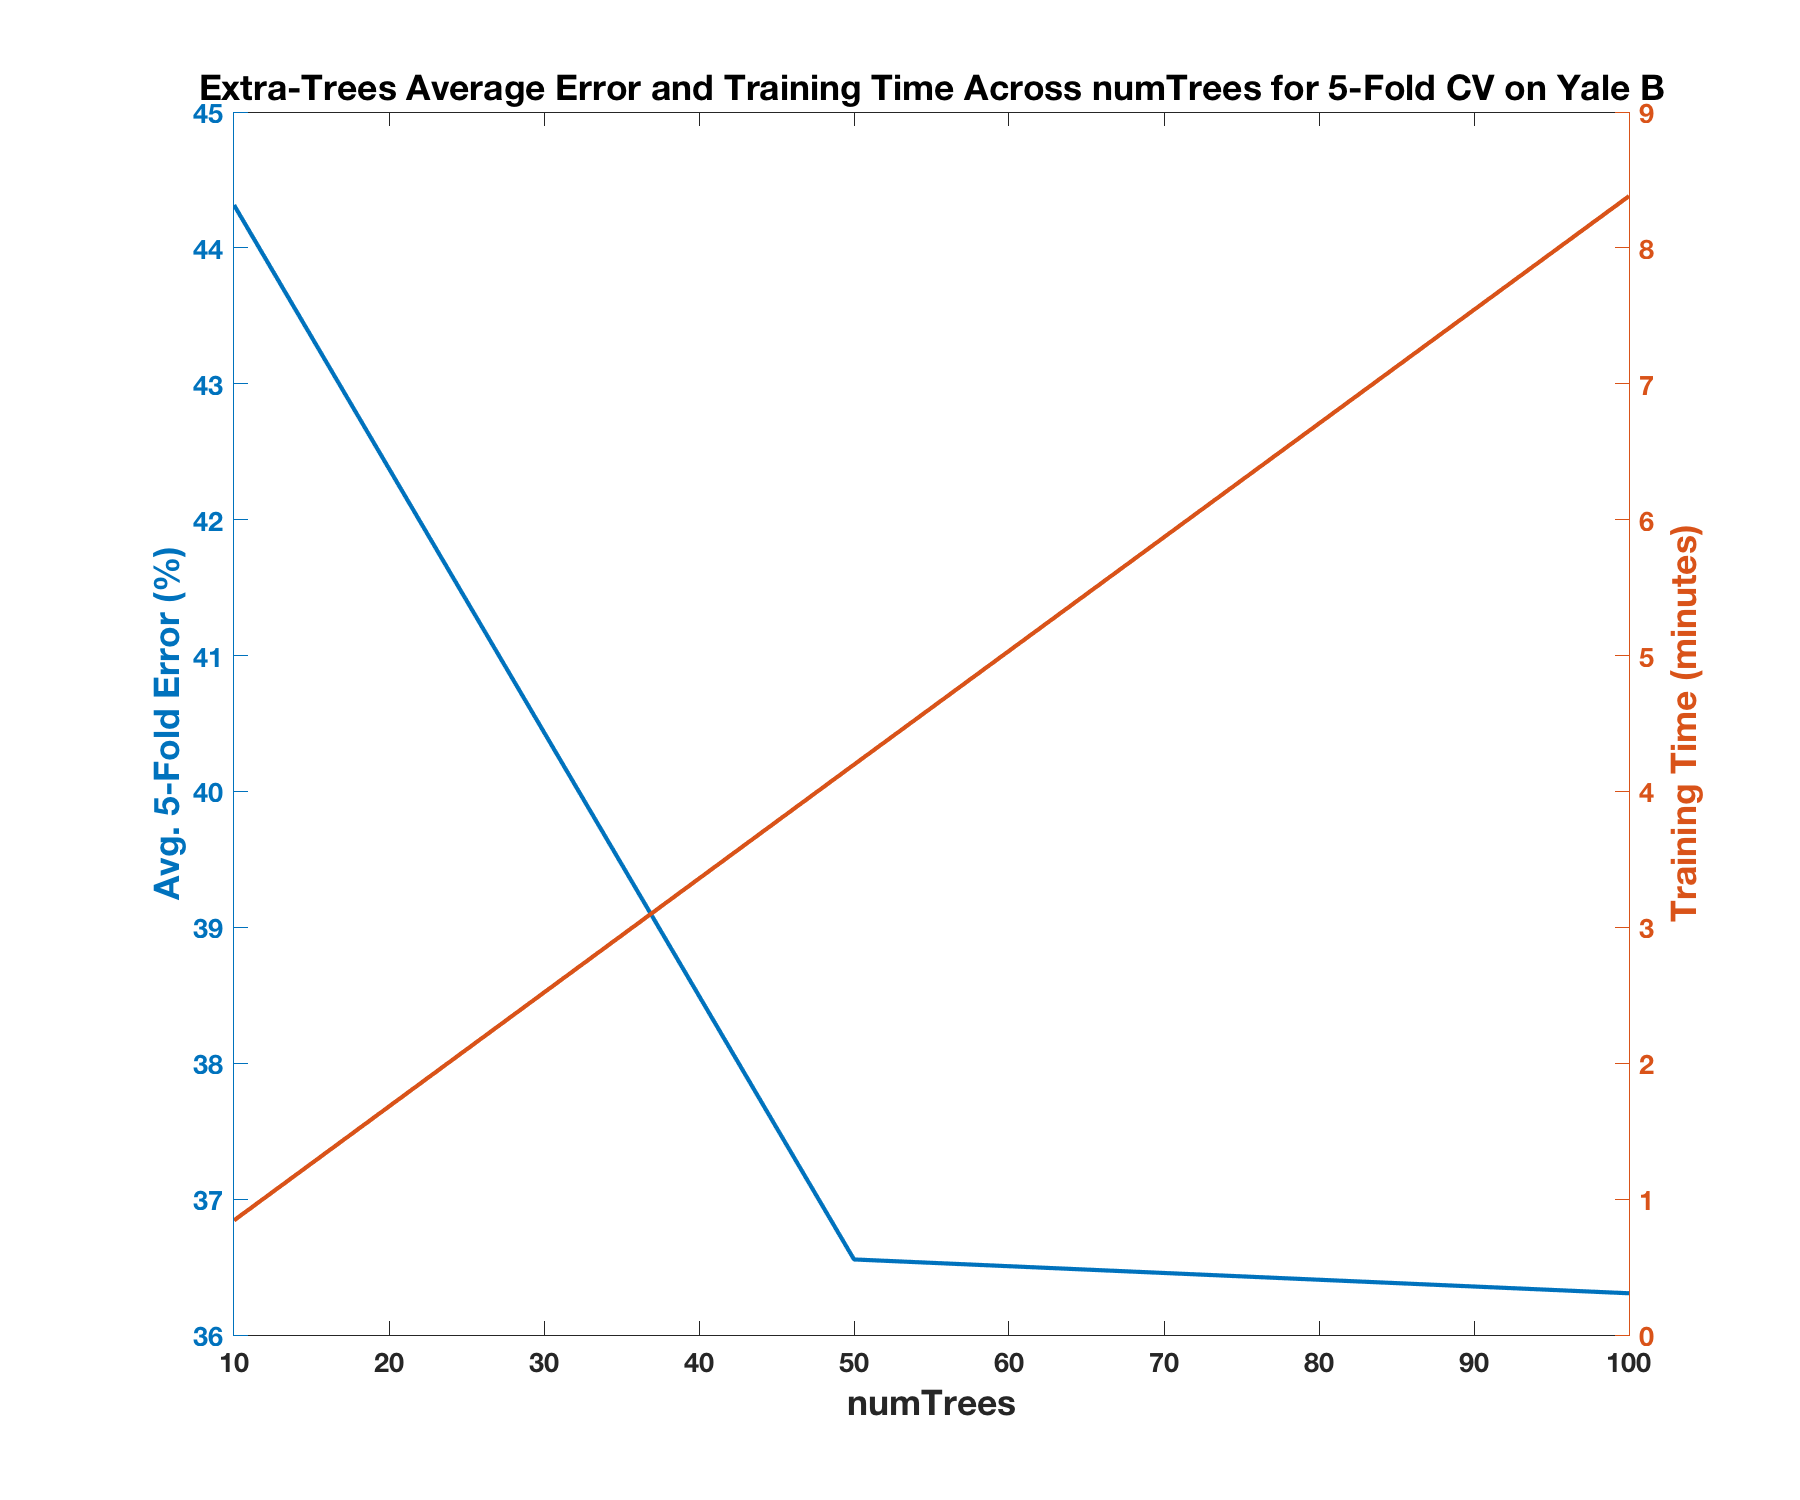
\includegraphics[width=0.5\columnwidth]{../images/cv_et_yaleb} }}
    \caption{Cross Validated Extra Tree Hyperparameter Results on MNIST (a) and Yale B (b).}
\end{figure}